\documentclass[12pt]{article}
%\usepackage{amsmath}
\usepackage{graphicx}
%\usepackage{enumerate}
\usepackage{natbib} %comment out if you do not have the package
\usepackage{url} % not crucial - just used below for the URL 
\usepackage{amsmath, amssymb}


%\pdfminorversion=4
% NOTE: To produce blinded version, replace "0" with "1" below.
\newcommand{\blind}{0}

% DON'T change margins - should be 1 inch all around.
\addtolength{\oddsidemargin}{-.5in}%
\addtolength{\evensidemargin}{-.5in}%
\addtolength{\textwidth}{1in}%
\addtolength{\textheight}{1.3in}%
\addtolength{\topmargin}{-.8in}%


\begin{document}

%\bibliographystyle{natbib}

\def\spacingset#1{\renewcommand{\baselinestretch}%
{#1}\small\normalsize} \spacingset{1}


%%%%%%%%%%%%%%%%%%%%%%%%%%%%%%%%%%%%%%%%%%%%%%%%%%%%%%%%%%%%%%%%%%%%%%%%%%%%%%

\if0\blind
{
  \title{\bf Combining model calibration and design}
  \author{Carl Ehrett\thanks{
    The authors gratefully acknowledge \textit{please remember to list all relevant funding sources in the unblinded version}}\hspace{.2cm}\\
    School of Mathematical and Statistical Sciences, Clemson University,\\
    D. Andrew Brown \\
    School of Mathematical and Statistical Sciences, Clemson University,\\
    Evan Chodora \\
    Department of Mechanical Engineering, Clemson University,\\
    Christopher Kitchens \\
    Department of Chemical and Biomolecular Engineering, Clemson University,\\
    and \\
    Sez Atamturktur \\
    Department of Architectural Engineering, Pennsylvania State University\\}
  \maketitle
} \fi

\if1\blind
{
  \bigskip
  \bigskip
  \bigskip
  \begin{center}
    {\LARGE\bf Title}
\end{center}
  \medskip
} \fi

\bigskip
\begin{abstract}
Abstract
\end{abstract}

\noindent%
{\it Keywords:}  Gaussian processes, material design, optimization, Pareto optimality, Uncertainty quantification, wind turbines
\vfill

\newpage
\spacingset{2} % DON'T change the spacing!
\section{Introduction}
\label{introduction}

%
The goal of traditional Kennedy-O'Hagan style calibration \citep[KOH, ][]{kennedy2001} is to find a posterior distribution on unknown parameters by calibrating a computer model using real-world observations of the modeled phenomenon.
%
By contrast, the design methodology of calibration to target outcomes (CTO) uses the KOH framework to find a posterior distribution on optimal input settings in the model by ``calibrating'' a computer model using artificial observations that reflect performance and cost targets for the modeled system.
%
The goal of the work described here is to combine KOH and CTO.
%
Call the resulting methodology DCTO, for dual calibration to target outcomes.

CTO as previously developed assumes, somewhat idealistically, that the computer model is already perfectly calibrated.
%
DCTO avoids this idealization.
%
Furthermore, when undertaking KOH, some areas of the model range may be of greater interest than others.
%
For example, one may be more interested in calibrating the model to be accurate in the optimal region of some design variable $\theta$ than elsewhere.
%
Undertaking dual calibration may allow us to focus our calibration efforts on such regions of interest, prioritizing them over other areas of the model range.
%

\section{The model}

%
Let $f$ be the model of interest, and partition its inputs as $(x,\theta_1,\theta_2)$ where $x$ denotes the known and/or controllable inputs, $\theta_1$ denotes the parameters targeted for KOH calibration, and $\theta_2$ denotes the input settings targeted for design via CTO.
%
If $f$ can be run quickly, then we use it directly in MCMC.
%
However, if it is computationally expensive, we employ a surrogate by setting a Gaussian process (GP) prior on $f$ with mean $m_0(x,t_1,t_2)$ and covariance function $C_0((x,t_1,t_2),(x',t_1',t_2'))$.
%
From here on in this discussion, assume that a GP surrogate is used for $f$.
%
Typically, there will be some systematic discrepancy between the output of $f$ and the true system, even if the true value of $\theta_1$ is used.
%
We model this discrepancy, between the true system and $f$ at the true value of $\theta_1$, with another GP prior $\delta_1$ having mean $m_1(x,t_2)$ and covariance function $C_1((x,t_2),(x',t_2'))$.
%
In addition to the discrepancy between $f$ and the true system, there may also be a systematic discrepancy between the true system and our performance/cost targets, particularly if the latter are especially optimistic.
%
We model this discrepancy using a GP prior with mean $m_2(x)$ and covariance function $C_2(x,x')$.
%
Notice that this discrepancy is between the true system at optimal settings for $\theta_2$ and $f$ using the true value of $\theta_1$ and the optimal settings for $\theta_2$.
%
In addition to systematic discrepancy between $f$ and reality, measurement error must be included in the model.
%
Thus let $\epsilon\sim N(0,\sigma^2)$ denote the (known) i.i.d.\ variance of (real) observations at any given values of $x,t_2$.
%
Finally, we assume that $\eta,\delta_1,\delta_2,$ and $\epsilon$ are all mutually independent.
%

%
A collection of simulation runs is needed to train the GP code surrogate.
%
Let $(\mathbf{x_s},\mathbf{t_{1s}},\mathbf{t_{2s}})$ be the design matrix for these simulation runs, and let $\mathbf{y_s}$ denote the output of these runs.
%
Similarly, let $\mathbf{y_r}$ be the real observations at $\mathbf{x_r},\mathbf{\theta_{2r}}$, and let $\mathbf {y_d}$ be a set of artificial ``observations'' reflecting our cost and performance targets at control settings $\mathbf {x_d}$.
%
Call $y_d$ the {\em target outcomes}.
%
Finally, let $\mathbf y = (\mathbf{y_s},\mathbf{y_r},\mathbf{y_d})^T$.
%
Then it follows that $\mathbf y\sim \mathrm{N}(\mathbf m,\mathbf C)$, where
\[
\mathbf m = \begin{pmatrix}
m_0(\mathbf{x_s},\mathbf{t_{1s}},\mathbf{t_{2s}})\\
m_0(\mathbf{x_r},\mathbf1\theta_1,\mathbf{t_{2r}}) + m_1(\mathbf{x_1},\mathbf{t_{2r}})\\
m_0(\mathbf{x_d},\mathbf1\theta_1,\mathbf1\theta_2) + m_1(\mathbf{x_d},\mathbf1\theta_2) + m_2(\mathbf{x_d})
\end{pmatrix},
\]
\[
\mathbf C = \begin{pmatrix}
\mathbf{C_{11}} & \mathbf{C_{12}} & \mathbf{C_{13}}\\
\mathbf{C_{21}} & \mathbf{C_{22}} & \mathbf{C_{23}}\\
\mathbf{C_{31}} & \mathbf{C_{32}} & \mathbf{C_{33}}
\end{pmatrix},
\]
\begin{align*}
\mathbf{C_{11}}&=C_0\left((\mathbf{x_s},\mathbf{t_{1s}},\mathbf{t_{2s}}),(\mathbf{x_s},\mathbf{t_{1s}},\mathbf{t_{2s}})\right)\\
\mathbf{C_{21}}&=C_0\left((\mathbf{x_s},\mathbf{t_{1s}},\mathbf{t_{2s}}),(\mathbf{x_r},\mathbf1\theta_1,\mathbf{t_{2r}})\right)\\
\mathbf{C_{31}}&=C_0\left((\mathbf{x_s},\mathbf{t_{1s}},\mathbf{t_{2s}}),(\mathbf{x_d},\mathbf1\theta_1,\mathbf1\theta_2)\right)\\
\mathbf{C_{12}}&=\mathbf{C_{21}}^T\\
\mathbf{C_{22}}&=C_0\left((\mathbf{x_r},\mathbf1\theta_1,\mathbf{t_{2r}}),(\mathbf{x_r},\mathbf1\theta_1,\mathbf{t_{2r}})\right) + C_1\left( (\mathbf{x_r},\mathbf{t_{2r}}),(\mathbf{x_r},\mathbf{t_{2r}}) \right) + \sigma_2 \mathbf I\\
\mathbf{C_{32}}&=C_0\left((\mathbf{x_r},\mathbf1\theta_1,\mathbf{t_{2r}}),(\mathbf{x_d},\mathbf1\theta_1,\mathbf1\theta_2)\right) + C_1\left( (\mathbf{x_r},\mathbf{t_{2r}}),(\mathbf{x_d},\mathbf1\theta_2) \right)\\
\mathbf{C_{13}}&=\mathbf{C_{31}}^T\\
\mathbf{C_{23}}&=\mathbf{C_{32}}^T\\
\mathbf{C_{33}}&=C_0\left((\mathbf{x_s},\mathbf1\theta_1,\mathbf1\theta_2),(\mathbf{x_s},\mathbf1\theta_1,\mathbf1\theta_2)\right) + C_1\left( (\mathbf{x_s},\mathbf1\theta_2),(\mathbf{x_s},\mathbf1\theta_2) \right) + C_2(\mathbf{x_d},\mathbf{x_d})
\end{align*}
%
Note that when $\mathbf{y_d}$ and $\mathbf{x_d}$ are empty and $\mathbf m, \mathbf C$ reduce respectively to their first two and upper two-by-two block elements, this is simply the KOH framework.
%
Thus, DCTO generalizes the KOH framework.
%

%
\section{Example with simulated data}
%
Consider the function of three inputs $f(x,t_1,t_2) = x / (t_2^{t_1-1}\exp(-0.75t_2)+1)$. 
%
Figure \ref{fig:example_output} shows the output of this function for $x=1$ over the range $(t_1,t_2)\in[1.5,4.5]\times[0,5]$.
%
% INSERT FIGURE 1 HERE
%
We arbitrarily set $\theta_1=2$ to be the ``true'' value of $t_1$.
%
For any value of $x$ and $t_1$, the optimal (minimizing) value of $t_2$ is $(4/3)(t_1-1)$, so we have $\theta_2=4/3.$
%
Figure \ref{fig:true_vals} shows the locations of the true and optimal values (respectively) of $\theta_1$ and $\theta_2$.
%
%INSERT FIGURE 2 HERE
%
There it is clear that the true value of $\theta_1$ is far from optimal -- if this value were within our control, its optimal value would be at the upper end of its support, at 4.5.
%
Thus $f$ showcases the ability of DCTO to perform simultaneously both calibration and design in the case when our ``truth-seeking'' goals and our design goals are in tension.
%

%
\subsection{Results}
% 
We used DCTO on four versions of the problem.
%
First, we assumed that $f$ is free from discrepancy -- i.e. that $f(x,\theta_1,t_2)$ is an unbiased estimator of the ``true'' system $g(x,t_2)$.
%
The other three versions each assume that $f$ suffers from some form of discrepancy.
%
Let $g_1,g_2,g_3$ denote the ``true'' systems in these three cases.
%
We set $g_1(x,t_2) = \left( \right) f(x,\theta_1,t_2)$ %HERE
%
To train the GP code surrogate, we drew a latin hypercube design of 250 points in the space of the model inputs.
%


\bigskip

%\begin{center}
%{\large\bf SUPPLEMENTARY MATERIAL}
%\end{center}
%
%\begin{description}
%
%\item[Title:] Brief description. (file type)
%
%\item[R-package for  MYNEW routine:] R-package �MYNEW� containing code to perform the diagnostic methods described in the article. The package also contains all datasets used as examples in the article. (GNU zipped tar file)
%%
%\item[HIV data set:] Data set used in the illustration of MYNEW method in Section~ 3.2. (.txt file)
%
%\end{description}

\bibliographystyle{Chicago}

\bibliography{lit_review}
\end{document}

\begin{figure}
\begin{center}
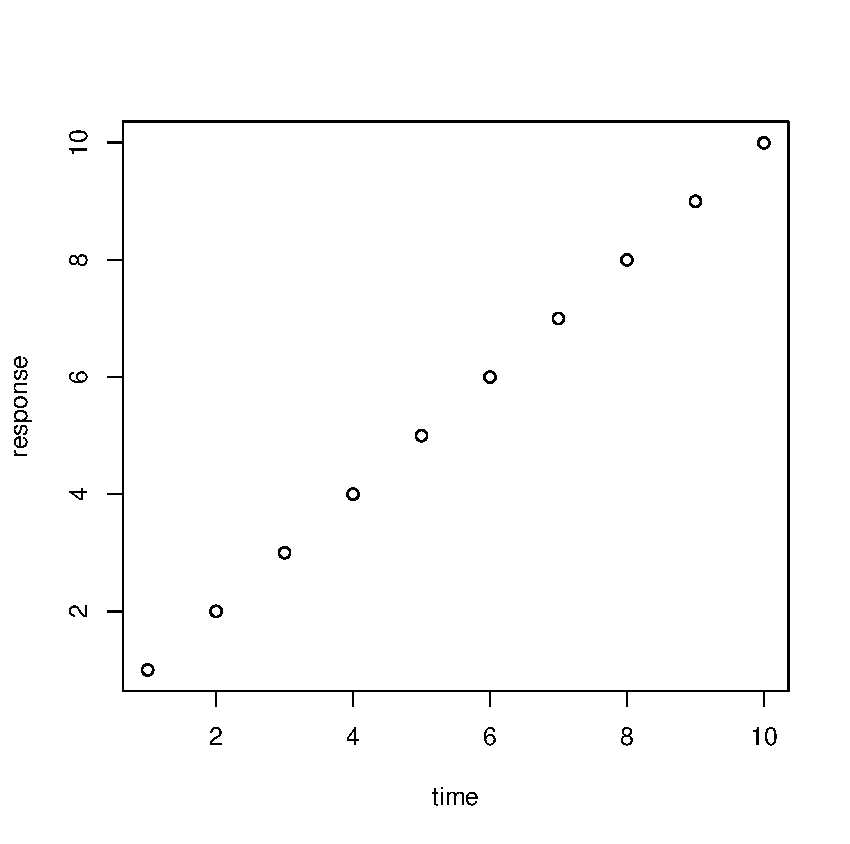
\includegraphics[width=3in]{fig1.pdf}
\end{center}
\caption{Consistency comparison in fitting surrogate model in the tidal
power example. \label{fig:first}}
\end{figure}

\begin{table}
\caption{D-optimality values for design $X$ under five different scenarios.  \label{tab:tabone}}
\begin{center}
\begin{tabular}{rrrrr}
one & two & three & four & five\\\hline
1.23 & 3.45 & 5.00 & 1.21 & 3.41 \\
1.23 & 3.45 & 5.00 & 1.21 & 3.42 \\
1.23 & 3.45 & 5.00 & 1.21 & 3.43 \\
\end{tabular}
\end{center}
\end{table}

\begin{itemize}
\item Note that figures and tables (such as Figure~\ref{fig:first} and
Table~\ref{tab:tabone}) should appear in the paper, not at the end or
in separate files.
\item In the latex source, near the top of the file the command
\verb+\newcommand{\blind}{1}+ can be used to hide the authors and
acknowledgements, producing the required blinded version.
\item Remember that in the blind version, you should not identify authors
indirectly in the text.  That is, don't say ``In Smith et. al.  (2009) we
showed that ...''.  Instead, say ``Smith et. al. (2009) showed that ...''.
\item These points are only intended to remind you of some requirements.
Please refer to the instructions for authors
at \url{http://www.tandfonline.com/action/authorSubmission?journalCode=utch20&page=instructions#.UieFdDafgx0}
\item If you have Supplementary Material (eg software, data, technical
proofs), identify them in the section below.  In early stages of the
submission process, you may be unsure what to include as supplementary
material.  Don't worry---this is something that can be worked out at later stages.
\end{itemize}
